%!TEX root = ../apese-rapport.tex
\section{Déroulement}
\subsection{Initialisation}
Afin de commencer notre projet, nous avons été sur Spring Initializer. Ce site est la version Web de l'outil intégré aux IDE tel que IntelliJ, Eclipse et NetBeans.

Il nous a permit de facilement choisir les dépendances du projet. Il faut savoir que Spring est un framework qui a pour but d'éviter de se prendre la tête avec la gestion des dépendances. Spring choisit les bonnes versions en veillant à la compatibilité entre elles.

\subsubsection{Configuration}

\paragraph{Generate}

Changeons l'option de base de \og{}Generate\fg{}, qui est par défaut sur \og{}Maven Project\fg{}, par \og{}Gradle Project\fg{}. C'est juste le moteur de production qui va servir à télécharger et installer les dépendances, compiler et lancer notre programme. Nous préférons utiliser Gradle à la place de Maven car il est beaucoup plus simple à comprendre et est plus puissant.

\paragraph{Project Metadata}

Dans la section \og{}Project Metadata, nous allons modifier le paquet de notre application ou \og{}Group\fg{}. On peut par exemple mettre \og{}be.heh\fg{}. Il s'agit généralement d'un nom de domaine écrit à l'envers.
L' \og{}Artifact\fg{} correspond au nom de l'application. Il ne contient pas d'espace et pas de caractères spéciaux.

\paragraph{Dépendances}

Afin de mener à bien ce projet, nous avons choisit les dépendances suivantes:

\begin{description}
	\item[Web] Permet d'utiliser notre application Spring comme une application Web.
	\item[JPA] Sert à faire la liaision entre nos objets Java et les la base de données tout en utilisant Hibernate.
	\item[JDBC] Est le pilote qui permet de faire la liaison entre notre projet Spring et la base de données.
	\item[PostgreSQL] Permet de se connecter à la base de données de type PostgreSQL.
	\item[OAuth2] Permet de faire le code qui va permettre d'envoyer le token et de gérer sa validité.
	\item[REST] Permet de faire le code de l'API Rest.
	\item[DevTools] Permet de compiler le code automatiquement de façon asynchrone à chaque sauvegarde afin de voir les modifications en direct dans le navigateur.
\end{description}

Nous sommes passé par ce service pour la simple et bonne raison que nous utilisons tous un éditeur différent. Le fait de passer par le site nous a permis de gagner un peu de temps.

\begin{figure}[ht]
	\centering
	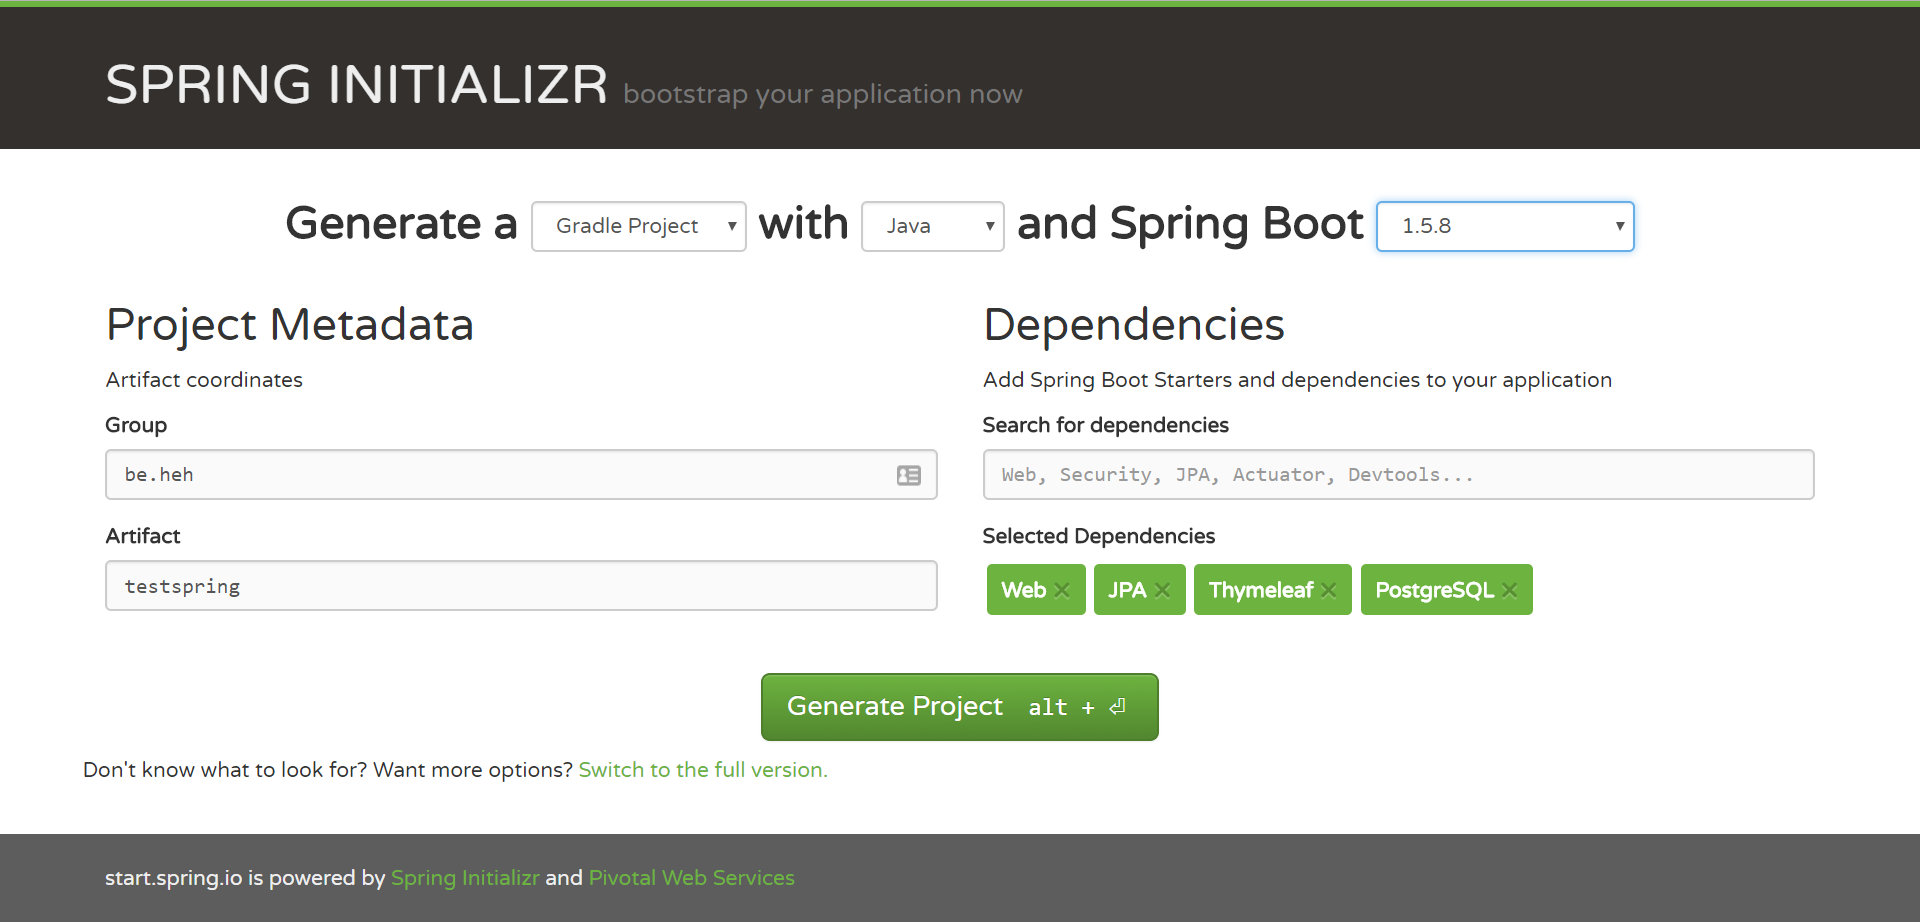
\includegraphics[width=\textwidth]{spring-start.PNG}
	\caption{Interface de Spring Initializer}
\end{figure}

\subsection{Répartition des tâches}
Afin de travailler plus efficacement, nous nous sommes réparti les différentes tâches. La partie front-end, plus conséquente, a été attribuée à Florian et à Alexandre. Quant à la partie back-end, elle a été attribuée à Guillaume. La partie base de données a été attribuée à Florian, car Alexandre avait déjà bien avancé sur le front-end.

\subsection{Organisation du code}
Afin de séparer correctement nos partie, nous avons voulu utiliser une méthode qui consiste à avoir un dossier qui contient toute la partie back-end et un dossier qui contient toute la partie front-end. Pour que tout compile correctement depuis la racine, nous avons créer des scripts et des fichiers de configurations qui permettent de spécifier les différents dossier à compiler ainsi que les sorties de compilation.

\subsection{Compilation et déploiement}
Afin de compiler et déployer notre application, nous avons utilisé Travis et Heroku comme demandé.

\subsubsection{Travis}

Travis est un outil super pratique en ligne qui permet de facilement compiler et déployer son code.

Pour le configurer, il suffit de créer le fichier \og{}\textit{\textbf{.travis.yml}} \fg{} à la racine du projet.

On a mis plusieurs options comme:

\begin{itemize}
	\item Désactiver les notifications par email (spam).
	\item Mettre la clé d'API générée sur le compte qui a créé la base de données.
	\item Spécifier le nom de l'application.
\end{itemize}

Voici le contenu mis:

\begin{lstlisting}
language: java

notifications:
    email: false

branches:
    only:
        - develop
        - master

deploy:
    provider: heroku
    api_key: "la clé API"
    app: lenomdelapp
\end{lstlisting}

\clearpage

Ensuite, nous avons été sur le site de TravisCI afin d'activer notre dépôt.

\begin{figure}[ht]
	\centering
	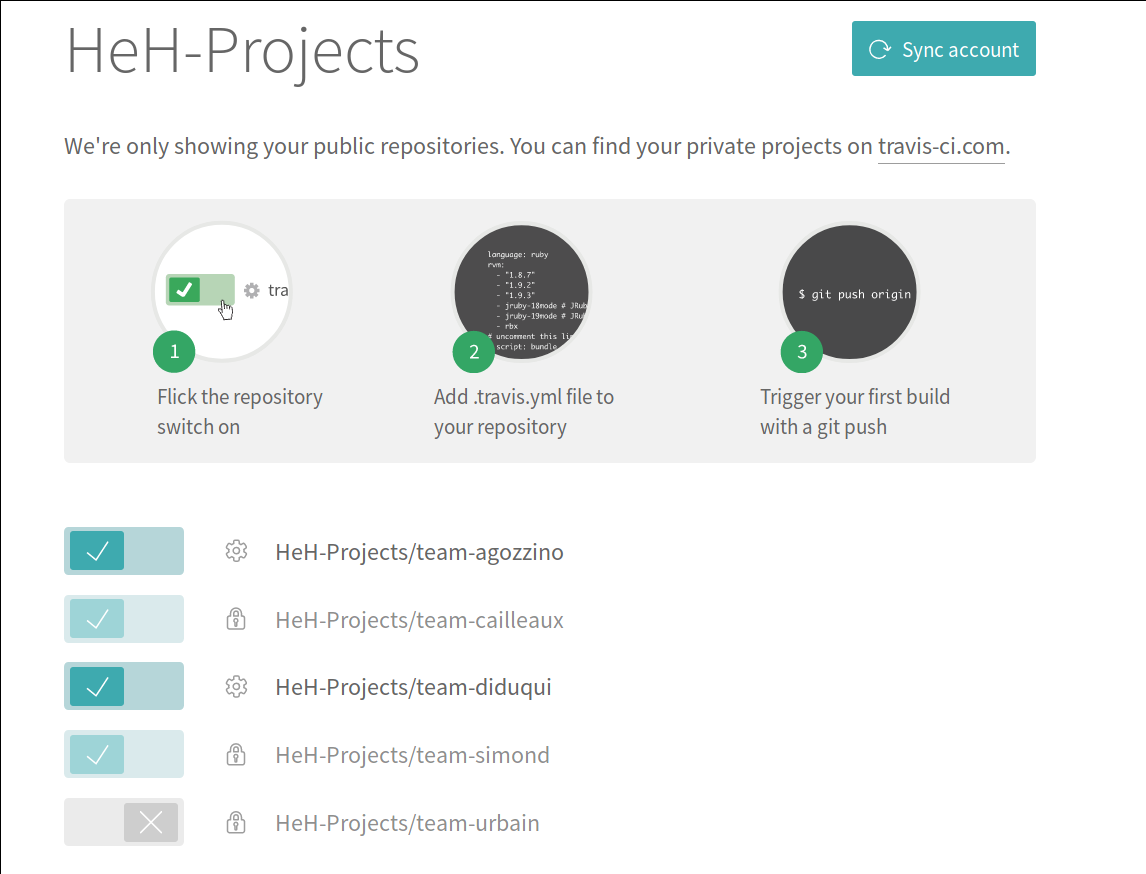
\includegraphics[width=\textwidth]{travis.png}
	\caption{Interface de Travis}
\end{figure}

Pour crypter notre clé, nous sommes aller sur le site \url{https://travis-encrypt.github.io/} et nous avons changé dans la configuration de Travis \og{}api\_key: \fg{} par \og{}api\_key: secure: \fg{}.

\clearpage

\subsection{Base de données}
\subsubsection{Outil de travail}
Afin de travailler sur la base de données, Florian a installé avec l'aide de Docker le programme PostgreSQL. \\
Il a récupéré une image afin de créer un container. \\
Il a par la suite créé des scripts qui lui ont permit de créer la base de données avec les tables.

\paragraph{Docker}

Vu qu'Heroku utilise le PostgreSQL, nous avons dû télécharger cette image:

\begin{lstlisting}
docker search postgresql
docker pull postgres
\end{lstlisting}
Installons l'image dans un container en partageant la base de données qui se trouve dans un dossier de notre ordinateur (\textit{ex:} C:/Users/test/database).

\begin{lstlisting}
docker run --name postgresDB -d -p 1000:5432 -v C:/Users/test/monapplication/database:/var/lib/postgresql postgres
\end{lstlisting}

On donne un nom au container afin de le manipuler plus facilement dans le futur. \\
Il est toujours conseillé de prendre les images officielles. \\
Pour lancer une invite de commande dans le container, il suffit de taper:

\begin{lstlisting}
docker exec -it postgresDB /bin/bash
\end{lstlisting}

Une fois dans le container, on peut par exemple se connecter à la base de données d'Heroku avec la commande suivante:

\begin{lstlisting}
psql -h hostname -U username -d database
\end{lstlisting}

On entre le mot de passe et nous sommes connectés à notre base de données.

\clearpage

\subsection{Back-end}
\subsubsection{Outil de travail}
Afin de faire correctement le back-end, Guillaume a voulu utiliser Eclipse, car bien qu'IntelliJ est mieux, quand nous allons sortir de l'école, nous n'aurons plus la licence afin de l'utiliser. \\
Vu le prix de cette dernière, il faut mieux s'habituer à utiliser des outils un peu moins performants mais qui restent gratuits.

\subsubsection{Organisation du code}
Afin de ne pas se faire surprendre par le nombre de fichiers, Guillaume a préféré utiliser des paquets. \\
En voici la liste :
\begin{description}
	\item[domain] Contient la partie API REST et objet de la base de données. On y retrouve les paquets suivants:
	\begin{description}
		\item[entities] Les objets de la base de données.
		\item[repositories] Les fonctions qui permettent de retourner ou modifier des données au format JSON, puis Java suivant l'URL utilisé.
	\end{description}
	\item[security] La partie sécurité du site avec le token.
	\item[web] Contient le contrôleur principal. Il sert juste à afficher l'application.
\end{description}

\subsubsection{Liaison avec la base de données}
Comme dit précédemment, nous avons utilisé JPA afin de se connecter à la base de données. Pour que celui-ci fonctionne correctement, nous avons dû créer une URL correcte. \\
En effet, l'URL données sur le site d'Heroku n'est pas valide quand on travaille avec le pilote JDBC. Il a donc fallu l'adapter. \\
Voici la configuration utilisée, à la page suivante :

\clearpage

\begin{lstlisting}
spring.datasource.url = jdbc:postgresql://Host:Port/Database?sslmode=require&user=User&password=Password
spring.datasource.username = User
spring.datasource.password = Password
spring.datasource.maxActive = 1
spring.datasource.maxIdle = 1
spring.datasource.minIdle = 0
spring.datasource.initialSize = 1
spring.datasource.removeAbandoned = true
spring.datasource.driver-class-name = org.postgresql.Driver
spring.jpa.database-platform = org.hibernate.dialect.PostgreSQLDialect
spring.jpa.show-sql = false
spring.jpa.hibernate.ddl-auto = none
spring.output.ansi.enabled = ALWAYS
server.port = 8080
\end{lstlisting}

La variable de configuration \og{}spring.jpa.hibernate.ddl-auto\fg{} est obligatoire, car on ne veut pas que Spring génère automatiquement les tables.

Pour les variables utilisées, nous avons été sur le site d'Heroku qui nous les fournis:
\begin{figure}[ht]
	\centering
	\includegraphics[width=\textwidth]{heroku-db-credentials.png}
	\caption{Partie base de données du site Heroku}
\end{figure}

\subsection{Front-end}
\subsubsection{Installation}

Pour la partie frontend, nous avons utilisé Angular. Pour commencer, on a installé Node.JS avec la commande suivante: 
\begin{lstlisting}
	npm install -g @angular/cli
\end{lstlisting}

Si jamais vous avez comme message d'erreur que \og{}user root does not have permission to access the dev dir \fg{}, il suffit de taper la commande suivante:
\begin{lstlisting}
npm install -g @angular/cli --unsafe-perm
\end{lstlisting}

\subsubsection{Commandes}

Voici la liste des commandes Angular utilisées:

\begin{description}
	\item[ng new nomduprojet] Créer un projet Angular
	\item[ng generate component nomducomponent] Créer un component
	\item[ng serve] Démarrer le serveur
\end{description}

Si jamais la commande \og{}ng serve\fg{} demande d'installer les node\_modules, il suffit d'effectuer la commande suivante dans le dossier de l'application Angular: npm install

\subsection{Intégration avec Spring}

Nous avons créé un fichier à la racine de l'application Angular et nous l'avons nommé \og{}proxy.conf.json \fg{}. Voici son contenu:

\begin{lstlisting}
{
    "/api": {
        "target": "http://localhost:8080",
        "secure": false
    }
}
\end{lstlisting}

\textbf{\textit{target}}, nous permet de spécifier le lien de notre application Spring avec le bon port.

\clearpage

Ensuite, nous avons édité le fichier \og{}package.json \fg{}. Nous avons modifié la partie \og{}scripts \fg{} comme ceci:

\begin{lstlisting}
"scripts": {
    "ng": "ng",
    "start": "ng serve --proxy-config proxy.conf.json",
    "build": "ng build -prod",
    "postbuild": "npm run deploy",
    "predeploy": "rimraf cheminVersLeDossierStatic && mkdirp cheminVersLeDossierStatic",
    "deploy": "cp -rf dist/** cheminVersLeDossierStatic",
    "test": "ng test",
    "lint": "ng lint",
    "e2e": "ng e2e"
},
\end{lstlisting}

Pour nous, le chemin vers le dossier static est \og{}../resources/static/ \fg{}.

En modifiant la partie \og{}start \fg{}, on spécifie à Angular de passer par le projet Spring pour utiliser la bonne API\@. \\
Ensuite, on spécifie à la partie \og{}build \fg{} que l'on veut une compilation de production. \\
On ajoute 3 options en dessous de cette ligne:

\begin{description}
	\item[postbuild] Lance le déploiement juste après la compilation.
	\item[predeploy] Supprime le dossier \og{}static \fg{} se trouvant dans \og{}resources \fg{} et le récrée. Cela permet de nettoyer tous les fichiers qui étaient dedans.
	\item[deploy] Permet de copier tous les fichiers empaquetés par Angular dans le dossier \og{}resources/static \fg{}. C'est là où Spring va rechercher les documents HTML\@.
\end{description}

Pour compiler l'application Angular afin de l'intégrer à Spring, il ne reste plus qu'à taper la commande suivante: \og{}ng run build \fg{}. Ainsi, on compile et empaquète notre projet Angular.

Dans Spring, il ne reste plus qu'à créer un \og{}controller \fg{} qui va permettre de lancer la page web générée précédemment en fonction de l'URL\@.

 